\documentclass[10pt,compress,usetitleprogressbar,mathserif]{beamer}
\usepackage[spanish, es-tabla,es-noquoting,es-noshorthands]{babel}
\usepackage{tikz} % Tikz (para el tema)
\usepackage{showexpl} % ???
\usepackage{amsthm}  %%
\usepackage{amsmath} % Matemáticas
\usepackage{amssymb} %%
\usepackage{graphicx} % Imágenes
\usepackage{adjustbox} % Tamaño de tablas
\graphicspath{{img/}} % Ruta de las imágenes
\usepackage{pgfplotstable} %Tablas
\usepackage{booktabs}% http://ctan.org/pkg/booktabs

\pgfplotstableset{ % Estilo de todas las tablas
sci zerofill,
column type/.add={|}{},
every last column/.style={column type/.add={}{|}},
every head row/.style={before row=\hline},
after row=\hline,
% tex.stackexchange.com/questions/110233
row predicate/.code={%
\pgfmathparse{int(mod(#1,5))}
\ifnum\pgfmathresult=0\relax
\else\pgfplotstableuserowfalse\fi}
}

\usepackage{listings} % Códigos

\definecolor{backg}{HTML}{F2F2F2}    % Fondo
\definecolor{comments}{HTML}{BDBDBD} % Comentarios
\definecolor{keywords}{HTML}{08388c} % Palabras clave
\definecolor{strings}{HTML}{0489B1}  % Strings

\lstset{
language=C++,
basicstyle=\ttfamily\small,
breaklines=true,
backgroundcolor=\color{backg},
keywordstyle=\color{keywords},
commentstyle=\color{comments},
stringstyle=\color{strings},
tabsize=2,
% Acentos, ñ, ¿, ¡ (tex.stackexchange.com/questions/24528)
extendedchars=true,
literate={á}{{\'a}}1 {é}{{\'e}}1 {í}{{\'i}}1 {ó}{{\'o}}1
         {ú}{{\'u}}1 {ñ}{{\~n}}1 {¡}{{\textexclamdown}}1
         {¿}{{?`}}1 {->}{{$\rightarrow$}}1 {=>}{{$\Rightarrow$}}1
}

% Solarized palette
\definecolor{solarizedBase03}{HTML}{002B36}
\definecolor{solarizedBase02}{HTML}{073642}
\definecolor{solarizedBase01}{HTML}{586e75}
\definecolor{solarizedBase00}{HTML}{657b83}
\definecolor{solarizedBase0}{HTML}{839496}
\definecolor{solarizedBase1}{HTML}{93a1a1}
\definecolor{solarizedBase2}{HTML}{EEE8D5}
\definecolor{solarizedBase3}{HTML}{FDF6E3}
\definecolor{solarizedYellow}{HTML}{B58900}
\definecolor{solarizedOrange}{HTML}{CB4B16}
\definecolor{solarizedRed}{HTML}{DC322F}
\definecolor{solarizedMagenta}{HTML}{D33682}
\definecolor{solarizedViolet}{HTML}{6C71C4}
\definecolor{solarizedBlue}{HTML}{268BD2}
\definecolor{solarizedCyan}{HTML}{2AA198}
\definecolor{solarizedGreen}{HTML}{859900}

\usetheme{epstfg}
\setbeamertemplate{note page}[compress]
\title{Práctica 2}
\author{Pablo Baeyens \and Antonio Checa \and Iñaki Madinabeitia \and José Manuel Muñoz \and Darío Sierra}
\date{Algorítmica}
\def\inline{\lstinline[basicstyle=\ttfamily]}

\begin{document}
\maketitle

\begin{frame}{Índice}
  \tableofcontents
\end{frame}
\section{El elemento en su posición}

\begin{frame}{El elemento en su posición}
\begin{description}
 \item[Entrada:] Vector \texttt{v} y su tamaño \texttt{n}
 \item[Salida:] Entero no negativo que indica el $i$ tal que $v[i]=i$ en caso de que exista o $-1$ en otro caso
\end{description}
\end{frame}

\subsection{Algoritmos}

\begin{frame}[fragile]{Algoritmo obvio}
Recorre cada elemento y comprueba si $v[i] = i$:
\lstinputlisting[firstline=23, lastline=28]{cpps/posicion.cpp}
\textbf{Eficiencia:} $O(n)$.
\end{frame}

\begin{frame}[fragile]{Algoritmo recursivo}
\lstinputlisting[firstline=60, lastline=72]{cpps/posicion.cpp}
\note{
\texttt{ajuste}: ajusta la comprobación en función de la posición.
El caso base utiliza el algoritmo obvio ajustado.}
\end{frame}

\begin{frame}{Casos del algoritmo}
El algoritmo considera \textbf{3} casos:
\begin{itemize}
  \item El elemento medio está en su posición
  \item $m < v[m]$. Basta comprobar el lado izquierdo:
  \[v[m + k] \geq v[m]+k>m+k\]
  \item $m > v[m]$. Basta comprobar el lado derecho:
  \[v[m - k] \leq v[m] -k < m - k\]
\end{itemize}
\end{frame}

\begin{frame}{Eficiencia teórica}
\[T(n) = \begin{cases} T(n/2) + O(1) & \mbox{si } n > 3 \\
O(1) & \mbox{si } n \leq 3 \end{cases}\]
\textbf{Eficiencia:} $O(\log(n))$.
\end{frame}

\begin{frame}[fragile]{Versión no recursiva}
\lstinputlisting[firstline=89, lastline=115]{cpps/posicion.cpp}
\textbf{Eficiencia:} $\mathbf{O(\log(n))}$
\end{frame}

\subsection{Determinación del umbral}

%% TODO: (Antonio) Estudio del umbral ¿algo más?

\begin{frame}{Umbral (tablas)}
\pgfplotstableread{dats/comp_umbral_posicion/posicion_t.dat}\posObvioCompUmbral
\pgfplotstableread{dats/comp_umbral_posicion/posicion_1.dat}\posDyVUmbralOne
\pgfplotstableread{dats/comp_umbral_posicion/posicion_1_umbral_2.dat}\posDyVUmbralTwo
\pgfplotstableread{dats/comp_umbral_posicion/posicion_1_umbral_3.dat}\posDyVUmbralThree
\pgfplotstableread{dats/comp_umbral_posicion/posicion_1_umbral_4.dat}\posDyVUmbralFour
\pgfplotstableread{dats/comp_umbral_posicion/posicion_1_umbral_5.dat}\posDyVUmbralFive
\pgfplotstablecreatecol[copy column from table={\posDyVUmbralOne}{[index] 1}] {par1} {\posObvioCompUmbral}
\pgfplotstablecreatecol[copy column from table={\posDyVUmbralTwo}{[index] 1}] {par2} {\posObvioCompUmbral}
\pgfplotstablecreatecol[copy column from table={\posDyVUmbralThree}{[index] 1}] {par3} {\posObvioCompUmbral}
\pgfplotstablecreatecol[copy column from table={\posDyVUmbralFour}{[index] 1}] {par4} {\posObvioCompUmbral}
\pgfplotstablecreatecol[copy column from table={\posDyVUmbralFive}{[index] 1}] {par5} {\posObvioCompUmbral}

\resizebox{\linewidth}{!}{
\pgfplotstabletypeset[
display columns/0/.style={column name=Tamaño},
display columns/1/.style={column name=Algoritmo Obvio},
display columns/2/.style={column name=Umbral 1},
display columns/3/.style={column name=Umbral 2},
display columns/4/.style={column name=Umbral 3},
display columns/5/.style={column name=Umbral 4},
display columns/6/.style={column name=Umbral 5},
skip rows between index={4}{20},
skip rows between index={25}{50}
]{\posObvioCompUmbral}}
\end{frame}

\begin{frame}{Umbral (gráficas)}
\begin{figure}[H]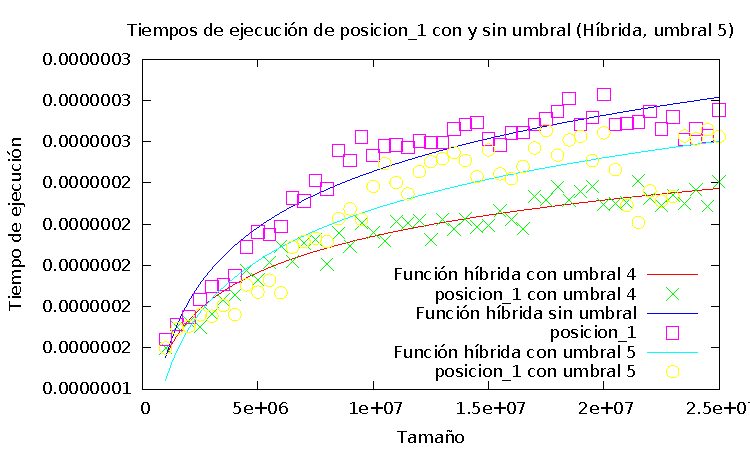
\includegraphics[width=13cm]{img/posicion_1_comparativa_umbral2.pdf} \centering
	\caption{Tiempos y funciones híbridas de umbrales 4 y 5}\end{figure}
\end{frame}

\begin{frame}{Umbral (gráficas)}
\begin{figure}[H]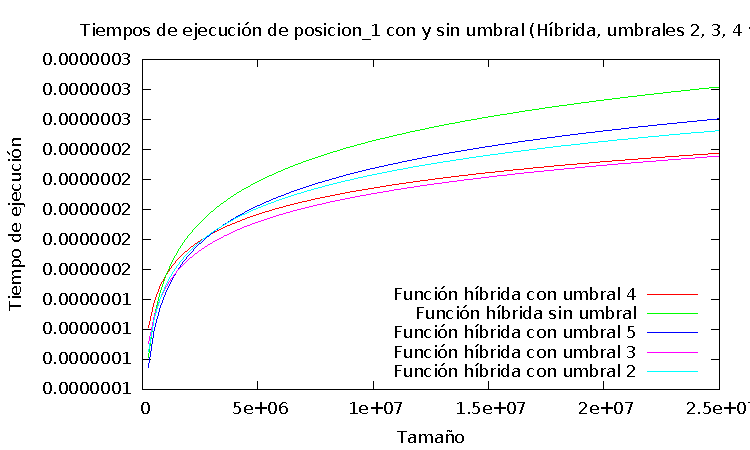
\includegraphics[width=13cm]{img/posicion_1_comparativa_umbral5.pdf} \centering
	\caption{Tiempos y funciones híbridas de umbrales 2, 3, 4 y 5}\end{figure}
\note{Como poner los 5 umbrales y sus híbridas haría que la gráfica fuera un poco caótica, hemos decidido poner una gráfica solo con las híbridas de los algoritmos, para que se vea la tendencia de los tiempos, que es lo que importa.}
\end{frame}

\begin{frame}{Umbral - Tamaño - Tiempo}
\begin{figure}[H]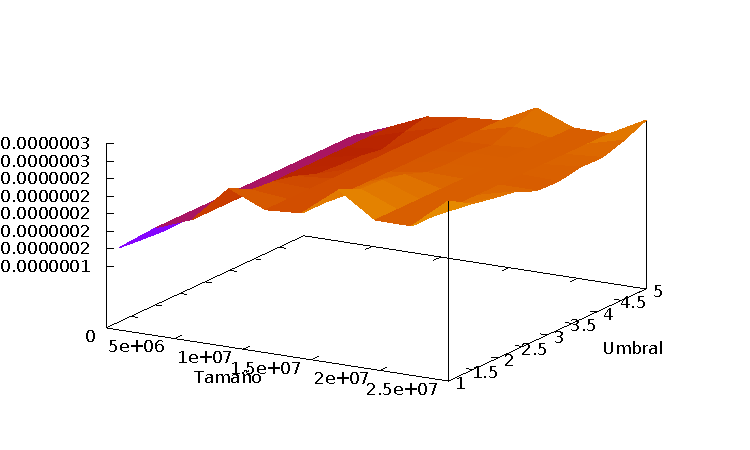
\includegraphics[width=13cm]{img/umbral_posicion.pdf} \centering
	\caption{Tiempos según Umbral y Tamaño}\end{figure}
\end{frame}

\subsection{Eficiencia empírica de los algoritmos}

\begin{frame}{Eficiencia empírica (tabla)}
\pgfplotstableread{dats/comp_umbral_posicion/posicion_t.dat}\posObvio
\pgfplotstableread{dats/comp_umbral_posicion/posicion_1.dat}\posDyV
%\pgfplotstableread{dats/comp_umbral_posicion/posicion_2.dat}\posDyVTwo
\pgfplotstablecreatecol[copy column from table={\posDyV}{[index] 1}] {par1} {\posObvio}
%\pgfplotstablecreatecol[copy column from table={\posDyVTwo}{[index] 1}] {par2} {\posObvio}

\pgfplotstabletypeset[
display columns/0/.style={column name=Tamaño},
display columns/1/.style={column name=Algoritmo Obvio},
display columns/2/.style={column name=Algoritmo DyV (rec)},
skip rows between index={25}{50}
%display columns/3/.style={column name=Algoritmo DyV (no rec)},
]{\posObvio}
\note{Aunque los algoritmos son rápidos para tamaños grandes, las funciones auxiliares utilizadas para la generación de muestras aleatorias que permitan medir el tiempo han dificultado la obtención de los datos. Los datos obtenidos pueden verse en la tabla.}
\end{frame}

\begin{frame}{Ajuste de las funciones (tabla)}
%% TODO: (¿?) Ajustes de las funciones
\end{frame}

\begin{frame}{Ajuste de las funciones (tabla)}
%% TODO: (Antonio) Gráfica con todos los algoritmos
\end{frame}

\subsection{Vectores con elementos repetidos}

En el caso de que tengamos elementos repetidos el razonamiento realizado para justificar el algoritmo divide y vencerás no es válido, y es sencillo encontrar ejemplos de vectores con elementos en su posición para los cuales nuestro algoritmo no funciona.

\begin{frame}{El algoritmo falla}
%% TODO: Poner bonico
\note{$v = [1,2,2]$. $1 <v[1]$, por lo que nuestro algoritmo comprobaría sólo el lado izquierdo ($[1]$) y no encontraría el elemento en la posición 2, que está en su posición.}
\end{frame}

\begin{frame}[fragile]{Algoritmo}
\lstinputlisting[firstline=126, lastline=150]{cpps/posicion.cpp}
Casi logarítmico cuando hay un elemento en su posición, y peor que lineal cuando no se encuentra.
\note{Como en una distribución uniforme sobre el rango de elementos en los que trabajamos la probabilidad de que un elemento caiga en su posición es bastante baja, por mucho que a veces sea logarítmico, no compensa las veces que es peor que lineal.}
\end{frame}

\begin{frame}{Comparación (tablas)}
  %%TODO: Comparación
\end{frame}

\begin{frame}{Comparación (gráficas)}
  %%TODO: Comparación
\end{frame}

\section{Comparación de preferencias}

\begin{frame}{Comparación de preferencias}
	\begin{description}
		\item[Entrada:] Vector de enteros \texttt{v} y su tamaño \texttt{n}
		\item[Salida:] Entero no negativo que indica el número de pares $i,j$ de posiciones del vector tales que $i < j$ y $v[i] > v[j]$
	\end{description}
\end{frame}

\subsection{Algoritmos}

\begin{frame}[fragile]{Algoritmo obvio}
	Recorre cada par de elementos $i,j : i < j$ y comprueba si $v[i] > v[j]$, sumando a un contador en tal caso:
	\lstinputlisting[firstline=24, lastline=32]{cpps/preferencias.cpp}
	\textbf{Eficiencia:} $O(n^2)$.
\end{frame}

\begin{frame}[fragile]{Algoritmo Divide y Vencerás}
	Se aplica \textit{mergesort} modificado: se obtiene el número de inversiones sumando:
	\begin{itemize}
		\item El número de pares invertidos en el subvector a la izquierda.
		\item El número de pares invertidos en el subvector a la derecha.
		\item El número de pares invertidos de subvectores distintos.
	\end{itemize}
	
	\pause
	Usando \textit{mergesort}, el tercer sumando se reduce a sumar cuántos elementos del primer subvector están pendientes de ser insertados en la mezcla cada vez que se inserta un elemento del segundo subvector.
	
	\pause
	
	Por debajo de un cierto umbral, usaremos el algoritmo de ordenación por inserción, que también puede usarse para contar el número de inversiones.
	No podemos usar el algoritmo obvio para esto porque, al mezclar, el \textit{mergesort} supone que los subvectores se encuentran ordenados, así que deben estar ordenados.
\end{frame}

% TODO: ¿Códigos? (son larguillos y divididos en trozos) ¿Presentar también inserción modificado? ¿Es necesario justificar que es O(n·log(n))?

\begin{frame}[fragile]{Ejemplo}
	\begin{tikzpicture}
		\node (T0) at (0,0) {$[5,2,3,4,1]_?$};
		\pause
		\node (Uu) at (-1,-1) {$[5,2,3]_?$};
		\node (Vu) at (1,-1) {$[4,1]_?$};
		\draw [->] (T0) -- (Uu);
		\draw [->] (T0) -- (Vu);
		\pause
		\node (Uo) at (-1,-2) {$[2,3,5]_2$};
		\node (Vo) at (1,-2) {$[1,4]_1$};
		\draw [->] (Uu) -- (Uo);
		\draw [->] (Vu) -- (Vo);
		\pause
		\node (T1) at (-3,-2) {$[\ ]_{2+1=3}$};
		\pause
		\node (T1) at (-3,-3) {$[1]_{3+3=6}$};
		\draw [->] (Vo) -- (T1);
		\node (Uo) at (-1,-3) {$[2,3,5]$};
		\node (Vo) at (1,-3) {$[4]$};
		\pause
		\node (T1) at (-3,-4) {$[1,2]_{6}$};
		\draw [->] (Uo) -- (T1);
		\node (Uo) at (-1,-4) {$[3,5]$};
		\node (Vo) at (1,-4) {$[4]$};
		\pause
		\node (T1) at (-3,-5) {$[1,2,3]_{6}$};
		\draw [->] (Uo) -- (T1);
		\node (Uo) at (-1,-5) {$[5]$};
		\node (Vo) at (1,-5) {$[4]$};
		\pause
		\node (T1) at (-3,-6) {$[1,2,3,4]_{6+1=7}$};
		\draw [->] (Vo) -- (T1);
		\node (Uo) at (-1,-6) {$[5]$};
		\node (Vo) at (1,-6) {$[\ ]$};
		\pause
		\node (T1) at (-3,-7) {$[1,2,3,4,5]_{7}$};
		\draw [->] (Uo) -- (T1);
		\pause
		\node (R) at (0, -7) {Inversiones: $7$};
		\draw [->] (T1) -- (R);
	\end{tikzpicture}
\end{frame}

% TODO: ¿Comentar algo del umbral? Tablas. Gráficas. Más tablas. Más gráficas.

\end{document}
